\section{Appendix}

\subsection{GANTT Chart}

Below is a GANTT Chart describing the idealised progression of the project over the next three years in order to complete the PhD project by September 2025. 

\begin{figure}[h]
    \centering
    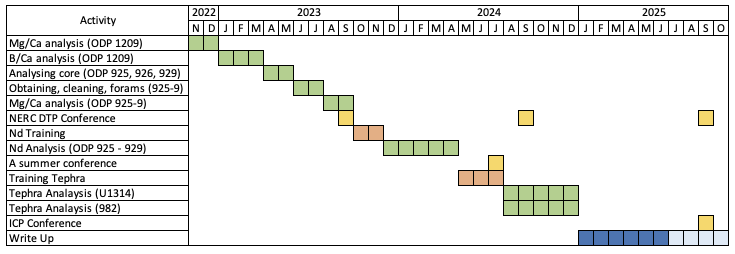
\includegraphics[width=\textwidth]{GANTT}
\end{figure}

\newpage

\subsection{Homogeneity of the Pacific Ocean}

The modern Pacific Ocean is relatively homogenous in $\delta^{18}\text{O}$ space. This can be seen by looking at the difference in oxygen isotopes between intermediate waters (defined as being lower than 2000 m depth) and deep waters (defined as being at at least 2500 m depth) in the North Pacific Ocean relative to other ocean basins (figure \ref{fig:oceans_sup}). The data come from core-top $\delta^{18}\text{O}$ measurements from \citep{schmittnerCalibrationCarbonIsotope2017}.

\begin{figure}[h]
    \centering
    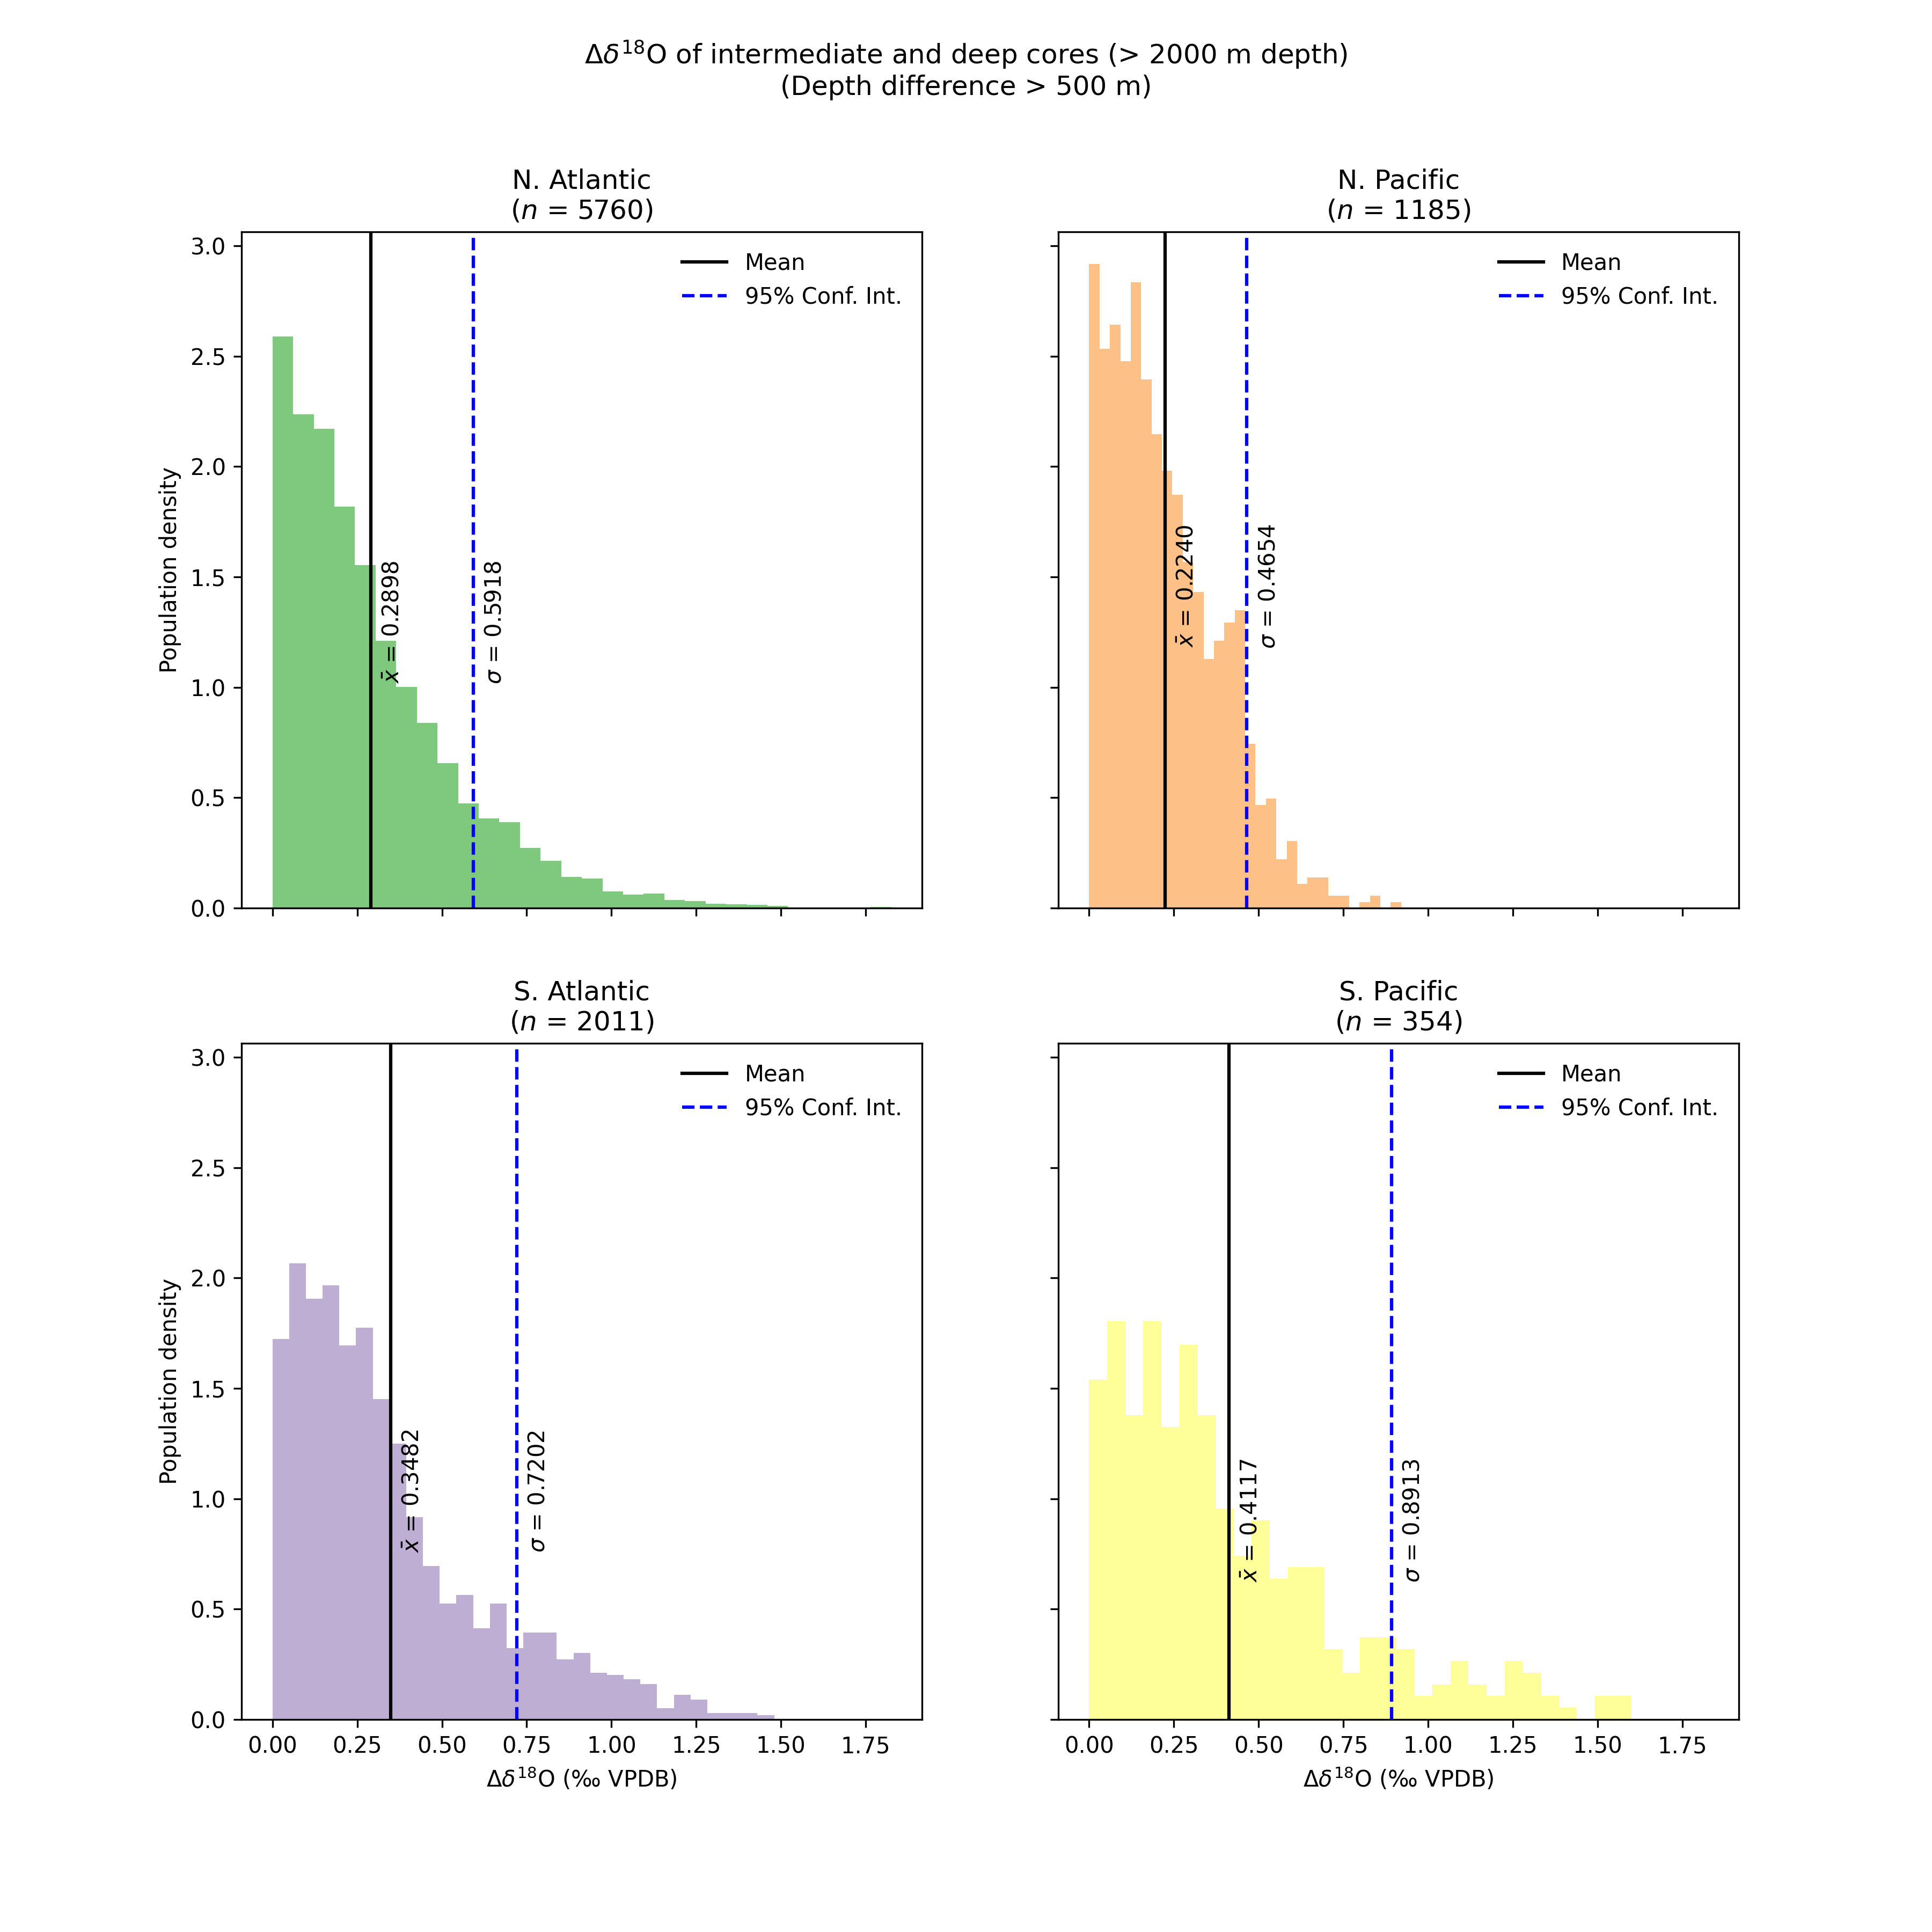
\includegraphics[width=0.8\textwidth]{oceans_sup}
    \caption{Histograms showing the difference in modern $\delta^{18}\text{O}$ measurements from core tops sampling intermediate (between 2000 - 2500 m depth) and deep (below 2500 m depth) for various ocean basins. Data from \citet{schmittnerCalibrationCarbonIsotope2017}]}
    \label{fig:oceans_sup}
\end{figure}

